\documentclass{article} % For LaTeX2e
\usepackage{nips14submit_e,times}
\usepackage{hyperref}
\usepackage{url}
\usepackage{graphicx}
\usepackage{float}
\usepackage{caption}
\usepackage{subcaption}
%\documentstyle[nips14submit_09,times,art10]{article} % For LaTeX 2.09


\title{CSE 546 Final Project Milestone:\\
	Feature Selection and Extraction for Noisy Data}


\author{
	Yuqing Ai \\
	\texttt{yuqingai@uw.edu} \\
	\And
	Jingchen Hu \\
	\texttt{jingchen@uw.edu} \\
}

% The \author macro works with any number of authors. There are two commands
% used to separate the names and addresses of multiple authors: \And and \AND.
%
% Using \And between authors leaves it to \LaTeX{} to determine where to break
% the lines. Using \AND forces a linebreak at that point. So, if \LaTeX{}
% puts 3 of 4 authors names on the first line, and the last on the second
% line, try using \AND instead of \And before the third author name.

\newcommand{\fix}{\marginpar{FIX}}
\newcommand{\new}{\marginpar{NEW}}

\nipsfinalcopy % Uncomment for camera-ready version

\begin{document}
	
	
	\maketitle
	
	\begin{abstract}
		In this report, we present several experimental results on the performances of feature selection and extraction algorithms on the Dexter dataset.
	\end{abstract}
	
	\section{Introduction}
	Feature selection and extraction are important preprocessing steps for machine learning tasks. These steps help reduce overfitting and enhance generalization by filtering / reconstructing the features to exclude the effects of irrelevant variables. In the meantime, they also reduce the feature space and make large scale training more efficient. In this project, we study a variety of feature selection and extraction algorithms.
	
	In this milestone report, we present several experimental results for the algorithms we implemented in the first half of the quarter. This includes the Principal Component Analysis for feature extraction, a filter approach: Fisher score filtering, and a wrapper approach: Sequential Forward Generation. We also tried LASSO regression for preprocessing.
	
	\section{Experiments}
	\subsection{Dataset}
	We use the the Dexter dataset (http://archive.ics.uci.edu/ml/datasets/Dexter) which was first used in a feature selection competition in NIPS 2003 workshop [4]. This dataset contains a lot of noisy data and irrelevant features (probes) intentionally added to make training harder, which is suitable for our purpose of testing the effectiveness of feature selection and extraction algorithms. Unfortunately, the organizers of the competition did not release the labels of the test data after the competition. Therefore, we use the training and validation data to do a 2-fold cross-validation.
	
	Dexter is a binary classification task with sparse integer features. The features are bag-of-word counts, which has a significantly larger dimensions than the number of training samples. The training and the validation data both contain 300 samples which are divided into two categories with exactly 150 samples each. The number of features is 20000 in the original dataset, and we would like to reduce the number to about $10\sim 300$.
	
	\subsection{Classifier}
	We use the LIBSVM library [2] to solve the final classification task after the initial feature selection and extraction phases. We use the linear kernel C-SVM with default value of the penalty parameter $C$ ($C=1$).
	
	\subsection{Methods}
	We implement several basic feature selection and extraction algorithms. Their performances are measured by the average accuracy in our 2-fold cross-validation.
    \subsubsection{Feature Extraction}
    \begin{enumerate}
      \item \textbf{Principal Component Analysis.} We project the feature vector of dimensions 20000 onto its first $k$ principal components. And then we use these $k$ dimensional short vectors as features to feed in the SVM algorithm. See Figure \ref{fig1} for the curve of accuracy when $k$ varies between $10$ and $300$, and \ref{fig2} for smaller $k$ between $3$ and $20$.
      \begin{figure}[H]
      \centering
      \begin{subfigure}{.5\textwidth}
      \centering
      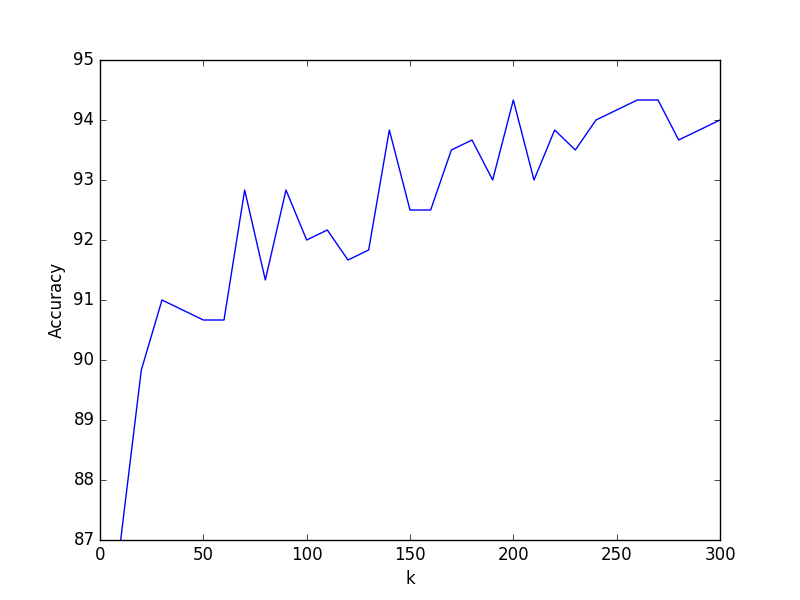
\includegraphics[width=\linewidth]{figure_1.png}
      \caption{When $10\leq k\leq 300$.}
      \label{fig1}
      \end{subfigure}%
      \begin{subfigure}{.5\textwidth}
      \centering
      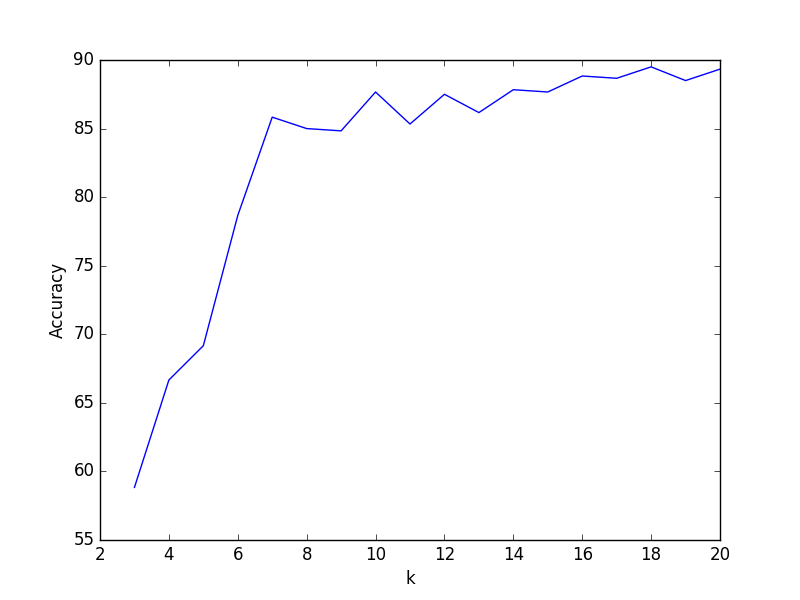
\includegraphics[width=\linewidth]{figure_2.png}
      \caption{When $3\leq k\leq 20$.}
      \label{fig2}
      \end{subfigure}
      \caption{The (Accuracy) - (Number of Dimensions) curve of PCA.}
      \label{fig1-2}
      \end{figure}
    \end{enumerate}
    
    \subsubsection{Feature Selection}
    \begin{enumerate}
          \item \textbf{Filter approach: Fisher Score.}
          Before running SVM, we calculate the Fisher score [3] for each feature and pick only the top $k$ features according to the score. See Figure \ref{fig3} and Figure \ref{fig4} for the accuracies when $k\in[10,300]$ and $k\in[3,20]$ accordingly.
          \begin{figure}[H]
          \centering
          \begin{subfigure}{.5\textwidth}
          \centering
          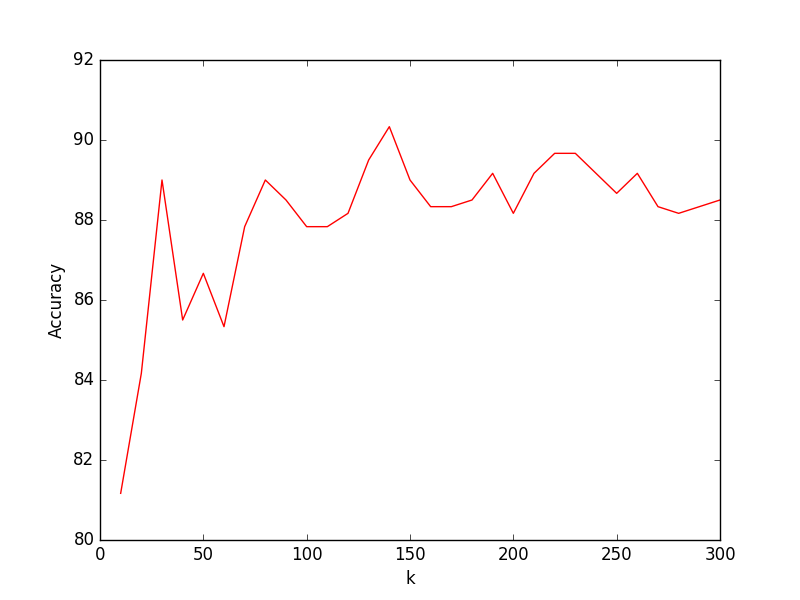
\includegraphics[width=\linewidth]{figure_3.png}
          \caption{When $10\leq k\leq 300$.}
          \label{fig3}
          \end{subfigure}%
          \begin{subfigure}{.5\textwidth}
          \centering
          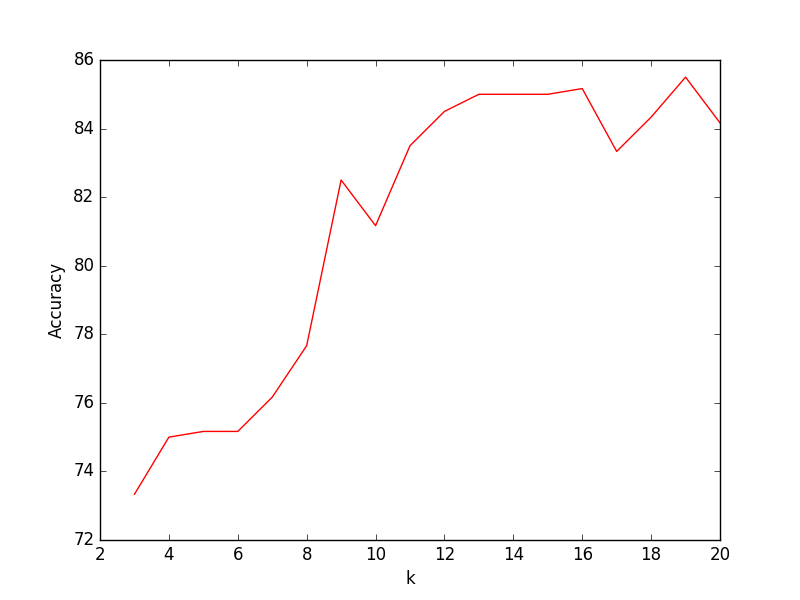
\includegraphics[width=\linewidth]{figure_4.png}
          \caption{When $3\leq k\leq 20$.}
          \label{fig4}
          \end{subfigure}
          \caption{The (Accuracy) - (Number of Selected Features) curve of Fisher score.}
          \label{fig3-4}
          \end{figure}

      \item \textbf{Wrapper Approach: Sequential Forward Generation.} 
      In the process of Sequential Forward Generation (SFG) [1], we start with an empty set of selected features and iteratively add the next best feature that yield the lowest error rate. We need to compute a new SVM classifier for each new feature we consider, which is time consuming for larger k values. See Figure \ref{fig5-5} for the curve of accuracy.
          \begin{figure}[H]
          \centering
          \begin{subfigure}{.5\textwidth}
          \centering
          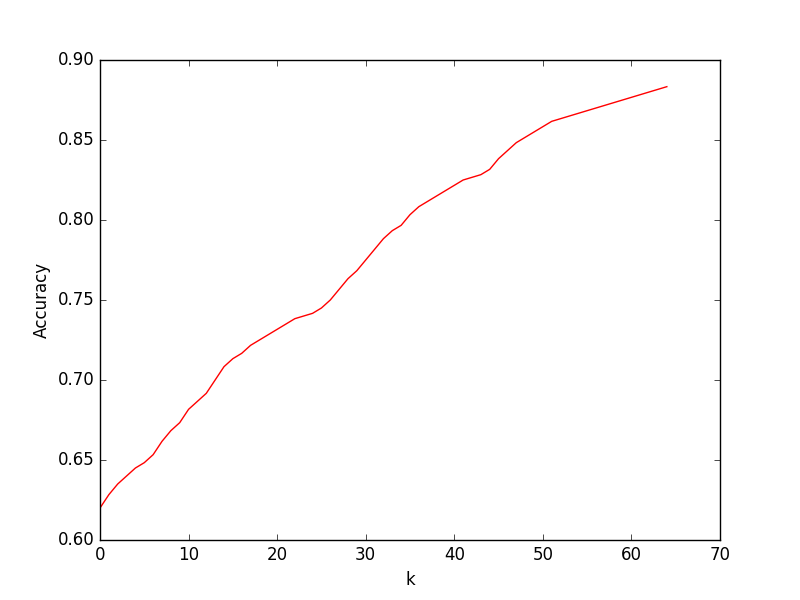
\includegraphics[width=\linewidth]{hillclimb.png}
          \label{fig5}
          \end{subfigure}
          \caption{The (Accuracy) - (Number of Selected Features) curve of SFG.}
          \label{fig5-5}
          \end{figure}
      \item \textbf{LASSO regression} applies L1 regularization that yields sparse weight vectors. We first run LASSO and tune $\lambda$ so that the error rate is the lowest. Then we rank the features by their magnitudes in the weight vector and run SVM on these features. See Figure \ref{fig6-6} for the curve of accuracy.
	      \begin{figure}[H]
          \centering
          \begin{subfigure}{.5\textwidth}
          \centering
          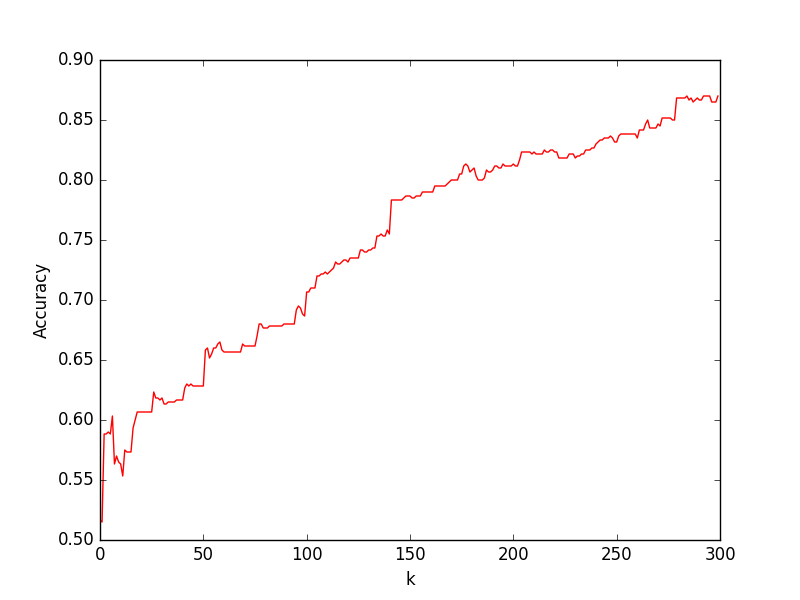
\includegraphics[width=\linewidth]{lasso.png}
          \label{fig6}
          \end{subfigure}
          \caption{The (Accuracy) - (Number of Selected Features) curve of LASSO feature selection.}
          \label{fig6-6}
          \end{figure}
	\end{enumerate}
	\section{Future Works}
	In the second half of the quarter, we plan to implement some more feature selection and extraction algorithms. We also would like to include some discussions and simple analysis of these algorithms in addition to experimental results in the final report. 
	\subsubsection*{References}
	
	\small{
        [1] Bolón-Canedo, V., Sánchez-Maroño, N., \& Alonso-Betanzos, A. (2013). A review of feature selection methods on synthetic data. Knowledge and information systems, 34(3), 483-519.
            
		[2] Chang, C. C., \& Lin, C. J. (2011). LIBSVM: a library for support vector machines. ACM Transactions on Intelligent Systems and Technology (TIST), 2(3), 27.
		
		[3] Duda, R. O., Hart, P. E., \& Stork, D. G. (2001). Pattern Classification, A Wiley-Interscience Publication John Wiley \& Sons.
        
        [4] Guyon, I., Gunn, S., Ben-Hur, A., \& Dror, G. (2004). Result analysis of the nips 2003 feature selection challenge. In Advances in neural information processing systems (pp. 545-552).
        
	}
	
\end{document}